\documentclass[a4paper,12pt]{report}

\usepackage[a4paper]{geometry}
\usepackage{amssymb,amsmath,amsthm}
\usepackage{graphicx}
\usepackage{url}
\usepackage{hyperref}
\usepackage{epsfig}
\usepackage[italian]{babel}
\usepackage{setspace}
\usepackage{thesis}
\usepackage{parskip}
\usepackage{booktabs}
\usepackage[utf8]{inputenc}

\newcommand{\partitioned}[2]{#1\slash\!\!#2}

\newtheorem{theorem}{Teorema}[chapter]
\newtheorem{definition}{Definizione}[chapter]

\begin{document}

% FRONTPAGE

\title{Iperminimizzazione di automi a stati finiti deterministici}
\author{Andrea TINELLI}
\dept{Corso di Laurea in Informatica} 
\anno{2023 - 2024}
\matricola{941800}
\relatore{Prof. Giovanni PIGHIZZINI}

% i think that this is not needed, but i have to verify
% with the professor, to re-enable it: remove the comment
% from the next line and from the thesis.sty file
% \correlatore{nome COGNOME}

% DEDICATIONS

\beforepreface
\prefacesection{}
{\hfill \Large {\sl dedicato a \dots}}

% PREFACE

\prefacesection{Prefazione}
Prefazione

% ORGANIZATION

\section{Organizzazione della tesi}
\label{organizzazione}
La tesi \`e organizzata come segue:
\begin{itemize}
\item nel Capitolo 1 ....
\end{itemize}

% THANKS TO

\prefacesection{Ringraziamenti}
grazie a 
\afterpreface

% CHAPTER 1

\chapter{Nozioni preliminari}
\label{cap1}

La teoria degli automi è uno dei principali e più antichi campi dell'informatica teorica. In questo capitolo
ne vengono presentati i concetti fondamentali. Per un'esposizione più completa il lettore è rimandato a \cite{HMU06}.

\section{Alfabeti, parole e linguaggi}

Un \emph{alfabeto}, generalmente indicato con la lettera $\Sigma$, è un insieme finito di simboli,
entità astratte non definite formalmente cui esempi possono essere lettere e numeri.

Una \emph{parola} (o \emph{stringa}) è una sequenza finita di simboli giustapposti, in particolare, una parola su un alfabeto $\Sigma$
è una sequenza finita di simboli appartenenti a $\Sigma$.

La \emph{lunghezza di una parola} $w$, indicata con $|w|$, è il numero di simboli che la compongono.
Caso particolare è la parola vuota, a cui per convenzione si fa riferimento con la lettera $\varepsilon$,
composta da zero simboli ($|\varepsilon| = 0$).

Un possibile esempio di alfabeto è $\Sigma = \{0, 1\}$, mentre una possibile parola su $\Sigma$ è
$w = 01$, dove $|w| = 2$.

Si è in grado a questo punto di introdurre il concetto di linguaggio.

\begin{definition}\label{def:lang}
  Un \emph{linguaggio} $L$ su un alfabeto $\Sigma$ è un insieme di parole su $\Sigma$, ovvero, un insieme di
  parole formate dalla giustappozione di simboli appartenenti a $\Sigma$.
\end{definition}

Due esempi particolari possono essere il linguaggio vuoto $L_\emptyset = \emptyset$ ed il linguaggio composto
solo dalla parola vuota $L_\varepsilon = \{\varepsilon\}$, puntualizzando il fatto che $L_\emptyset \neq L_\varepsilon$,
infatti $|L_\emptyset| = 0$ mentre $|L_\varepsilon| = 1$.

Convenzionalmente, fissato un alfabeto $\Sigma$, viene indicato con $\Sigma^*$ il linguaggio composto da tutte
le parole su $\Sigma$, compresa la parola vuota.

Sia $\Sigma = \{a, b\}$, allora $\Sigma^* = \{\varepsilon, a, b, aa, ab, ba, bb, aaa, \dots\}$.

\section{Automi a stati finiti}

In generale, un automa è un modello matematico di una macchina che esegue delle operazioni predefinite.

Una delle principali tipologie di automi è quella degli automi a stati finiti (FSA), questi, sono sistemi
con un numero finito di input, che possono trovarsi in un numero finito di configurazioni interne chiamate stati. 
In questa categoria rientrano gli automi a stati finiti deterministici (DFA) e gli automi a stati finiti 
non deterministici (NFA).

\begin{definition}
  \label{def:dfa}
  Un \emph{automa a stati finiti deterministico} è una quintupla $A = (Q, \Sigma, \delta, \allowbreak q_I, F)$
  dove $Q$ denota un insieme finito di stati, $\Sigma$ un alfabeto, $\delta: Q \times \Sigma \rightarrow Q$ 
  la funzione di transizione, $q_I \in Q$ lo stato iniziale e $F \subseteq Q$ l'insieme degli stati finali.
\end{definition}

La funzione di transizione $\delta$ può essere estesa per essere applicata a parole. Si definisce dunque
$\hat{\delta}: Q \times \Sigma^* \rightarrow Q$ dove $\hat{\delta}(q, w)$ è lo stato in cui l'automa si trova,
partendo dallo stato $q$, dopo aver letto la parola $w$. Più formalmente, $\hat{\delta}(q, \varepsilon) = q$ e
$\hat{\delta}(q, w\sigma) = \delta(\hat{\delta}(q, w), \sigma)$ per ogni $w \in \Sigma^*$ e $\sigma \in \Sigma$.

Una comune rappresentazione della funzione di transizione è quella in forma tabellare, chiamata tabella di transizione,
nella quale le righe corrispondono agli stati, le colonne ai possibili simboli in ingresso ed il generico elemento
di riga $q$ e colonna $\sigma$ allo stato $\delta(q, \sigma)$. Lo stato iniziale e gli stati finali sono evidenziati
rispettivamente con $\rightarrow$ e $*$.

Generalmente, gli automi a stati finiti vengono rappresentanti graficamente attraverso grafi orientati.
In tale rappresentazione gli archi corrispondono alle transizioni e i nodi agli stati, tra i quali, lo stato iniziale è
evidenziato con un arco in ingresso privo di origine mentre gli stati finali sono evidenziati con un doppio cerchio.

Un esempio di automa a stati finiti deterministico è mostrato in Figura \ref{fig:dfa}, in tale caso,
$Q = \{A, B, C, D, E, F, G, H\}$, $\Sigma = \{a, b\}$, $q_I = A$ e $F = \{E, G, H\}$, mentre
la funzione di transizione $\delta$ è mostrata in Tabella \ref{tab:transitions}.

\begin{definition}
  \label{def:reg-lang}
  Sia $A = (Q, \Sigma, \delta, q_I, F)$ un automa a stati finiti deterministico, si definisce il \emph{linguaggio
  riconosciuto} da $A$ come $L(A) = \{w \in \Sigma^* \mid \hat{\delta}(q_I, w) \in F\}$, ovvero, come
  il linguaggio composto da tutte le parole $w \in \Sigma^*$ che portano dallo stato iniziale $q_I$ ad
  uno stato $q \in F$.
\end{definition}

Gli automi a stati finiti non deterministici sono simili ai DFA, la differenza principale risiede nella
funzione di transizione che è definita come $\delta: Q \times \Sigma \rightarrow 2^Q$ che ne cambia di
conseguenza anche il modo di processare gli input. In questo modo, partendo dallo stato iniziale e leggendo
una parola $w$ è possibile raggiungere più stati. La parola è accettata se almeno uno degli stati raggiunti è
finale.

Data la non rilevanza degli NFA per il proseguo della trattazione, maggiori dettagli, per i quali il lettore è
nuovamente rimandato a \cite{HMU06}, sono omessi. Si ritiene tuttavia importante puntualizzare come gli automi
a stati finiti non deterministici siano equivalenti a quelli deterministici, ovvero, per ogni NFA esiste un
DFA che riconosce lo stesso linguaggio e viceversa.

\begin{figure}[!htb]
  \centering
  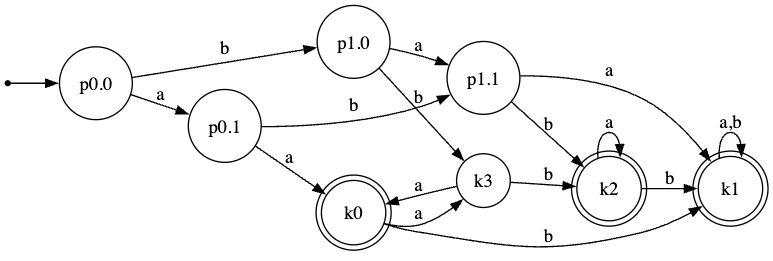
\includegraphics[width=0.7\linewidth]{dfa.png}
  \caption{\label{fig:dfa}Un esempio di automa a stati finiti deterministico.}
\end{figure}

\begin{table}[!htb]
  \centering
  \begin{tabular}{r|c|c}
    \toprule
                      & $a$ & $b$ \\
    \midrule
    $\rightarrow A$   & $B$ & $C$ \\
    $B$               & $E$ & $D$ \\
    $C$               & $D$ & $F$ \\
    $D$               & $H$ & $G$ \\
    $*E$              & $F$ & $H$ \\
    $F$               & $E$ & $G$ \\
    $*G$              & $G$ & $H$ \\
    $*H$              & $H$ & $H$ \\
    \bottomrule
  \end{tabular}
  \caption{\label{tab:transitions}Tabella di transizione dell'automa in Figura \ref{fig:dfa}.}
\end{table}

\section{Minimizzazione di DFA}
\label{min-dfa}

Uno dei problemi di maggiore interesse nel campo della teoria degli automi è quello riguardante la minimizzazione di 
automi a stati finiti deterministici. Il problema consiste, dato un automa $A = (Q, \Sigma, \delta, q_I, F)$,
nel trovare un automa $A' = (Q', \Sigma, \delta', q_I', F')$ tale che $L(A') = L(A)$ e $||Q'||$ sia minimo.

Il concetto alla base della minimizzazione è quello di equivalenza tra stati:

\begin{definition}
  \label{def:eq-states}
  Due stati $q_A$ e $q_B$ sono detti \emph{equivalenti}, denotato con $q_A \equiv q_B$, 
  se $\forall w \in \Sigma^*$, $\hat{\delta}(q_A, w) \in F$ se e solo se $\hat{\delta}(q_B, w) \in F$.
  Specularmente, due stati $q_A$ e $q_B$ non equivalenti sono detti distinguibili.
\end{definition}

\begin{theorem}
  \label{th:eq-rel-states}
  "$\equiv$" è una relazione di equivalenza, ovvero, è riflessiva, simmetrica e transitiva.
\end{theorem}

L'importanza dell'equivalenza tra stati è evidente nel momento in cui si considera che
due stati equivalenti, possono essere sostituiti da un singolo stato che si comporti come entrambi.
La diretta conseguenza risiede nel fatto che, dato un automa di partenza $A = (Q, \Sigma, \delta, q_I, F)$, 
siano $q_A, q_B \in Q$ tali che $q_A \equiv q_B$, è possibile costruire un automa $A' = (Q', \Sigma, \delta', q_I', F')$,
con $||Q'|| < ||Q||$ e $L(A') = L(A)$, facendo collassare gli stati $q_A$ e $q_B$ in un singolo stato $q'$, ovvero, definendo
$Q' = Q \setminus \{q_A, q_B\} \cup \{q'\}$ e la funzione di transizione $\delta'$
in modo che tutte le transizioni in ingresso a $q_A$ e $q_B$ vengano reindirizzate a $q'$ e che
$\delta'(q', \sigma) = \delta(q_A, \sigma)$ per ogni $\sigma \in \Sigma$, prestando particolare attenzione,
se necessario, anche alla conseguente ridefinizione dello stato iniziale e degli stati finali in $A'$.

Il teorema \ref{th:eq-rel-states} permette di estendere il risultato sopra riportato ad un numero arbitrario di
stati equivalenti, più formalmente, siano $q_1, q_2, \dots, q_n \in Q$ con $n \in \mathbb{N}$ tali che
$q_1 \equiv q_2 \equiv \dots \equiv q_n$, allora è possibile collassare gli stati $q_1, q_2, \dots, q_n$ in un
singolo stato $q'$ mantenendo il linguaggio riconosciuto dall'automa inalterato.

Grazie all'idea di equivalenza tra stati, è possibile definire l'equivalenza tra automi: siano
$A_1 = (Q_1, \Sigma, \delta_1, q_{I_1}, F_1)$ e $A_2 = (Q_2, \Sigma, \delta_2, q_{I_2}, F_2)$ due DFA, 
$A_1$ è detto \emph{equivalente} ad $A_2$, denotato con $A_1 \equiv A_2$, se $q_{I_1} \equiv q_{I_2}$.
É banale osservare che, se $A_1 \equiv A_2$, questi accettano gli stessi input, pertanto $L(A_1) = L(A_2)$.

Ricordando inoltre che una classe di equivalenza è un sottoinsieme della partizione $P$ di un insieme $S$ determinata da
una relazione di equivalenza $R$ su $S$ \cite{Ros18}, si introduce il concetto di \emph{insieme quoziente},
denotato da $S \slash R$, come l'insieme delle classi di equivalenza di $R$ su $S$.

\begin{theorem}
  \label{th:min-dfa}
  Sia $A = (Q, \Sigma, \delta, q_I, F)$ un automa a stati finiti deterministico, $A$ è detto \emph{minimo}
  (o \emph{minimizzato}) se non esiste un automa $A' = (Q', \Sigma, \delta', q_I', F')$ tale che $A \equiv A'$ e $||Q'|| < ||Q||$.
\end{theorem}

Queste nozioni permettono di fornire quella che è la soluzione al problema della minimizzazione di un automa a
stati finiti deterministici.

Dato un automa $A = (Q, \Sigma, \delta, q_I, F)$, l'automa $A' = (Q', \Sigma, \delta', q_I', F')$ ottenuto, dapprima
rimuovendo gli stati irraggiungibili in $A$, e successivamente $\forall Q_i \in \partitioned{Q}{\equiv}$ collassando gli stati
in $Q_i$ in un singolo stato $q_i \in Q_i$ scelto arbitrariamente, è equivalente ad $A$ e $||Q'||$ è minimo.
$A'$ corrisponde quindi all'automa $A$ minimizzato.

\begin{theorem}
  \label{th:unique-min-dfa}
  L'automa minimo $A'$ ottenuto come descritto sopra è unico, questo significa che a meno di isomorfismi,
  non esiste un automa $A''$ tale che $A'' \equiv A'$ e $A'' \neq A'$.
\end{theorem}

Prendendo come esempio l'automa in Figura \ref{fig:dfa}, si procede alla sua minimizzazione seguendo
la procedura sopra descritta. L'automa risulta essere privo di stati irraggiungibili,
pertanto si procede da subito con il calcolo del partizionamento di $Q$ in classi di equivalenza,
che risulta essere
$\partitioned{Q}{\equiv} \ = \{ \{A\}, \{B\}, \{C\}, \{D\}, \{E\}, \{F\}, \{G, H\}\}$.
Si passa quindi al collasso degli stati, in particolare, gli unici stati equivalenti risultano essere
$G$ e $H$ che vengono sostituiti da un unico stato $G$, ottenendo l'automa in Figura \ref{fig:minified-dfa}.

In ultima istanza, si sottolinea come sia ben noto un algoritmo per la minimizzazione di automi a stati finiti deterministici, 
l'algoritmo di Hopcroft \cite{Hop71}, che permette, partendo da un DFA in ingresso, di ottenere l'automa minimo in tempo $n \cdot log(n)$.

\begin{figure}[!htb]
  \centering
  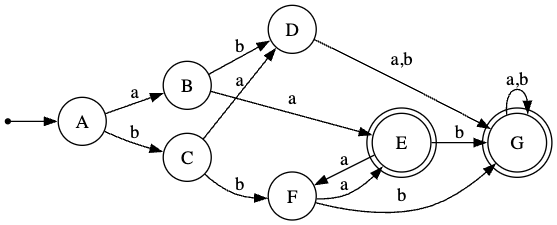
\includegraphics[width=0.7\linewidth]{minified-dfa.png}
  \caption{\label{fig:minified-dfa}L'automa in Figura \ref{fig:dfa} minimizzato.}
\end{figure}

% CHAPTER 2

% SKELETON

% \chapter{Iperminimizzazione di DFA}
% \label{cap2}
% 
% Come visto nella sezione \ref{min-dfa}
% 
% \section{Definizione del problema}
% 
% \section{Tecniche di iperminimizzazione}
% 
% \subsection{Algoritmo di Badr, Geffert e Shipman}
% 
% \subsection{Algoritmo di Badr}
% 
% \subsection{Algoritmo di Holzer e Maletti}


% CHAPTER 3

% SKELETON

% \chapter{Implementazione delle tecniche di iperminimizzazione}
% \label{cap3}
% 
% \section{Scelte implementative}
% 
% \section{Strutture comuni}
% 
% \section{Algoritmo di Badr, Geffert e Shipman}
% 
% \section{Algoritmo di Badr}
% 
% \section{Algoritmo di Holzer e Maletti}

% CHAPTER 4

% SKELETON

% \chapter{Risultati sperimentali}
% \label{cap4}
% 
% \section{Generazione di DFA}
% 
% \section{Risultati}

% BIBLIOGRAPHY

\bibliographystyle{alpha}
\bibliography{bibliography}

\end{document}